\chapter{Vita}

% Change the descriptions accordingly

%\foreach \n in {1,...,\numberOfAuthors}{
%\vfill


\includegraphics[width=0.2\columnwidth]{Castillo}
\documentAuthor{firstname1} \ \documentAuthor{surname1} \ is currently studying B. S. Computer Engineering in De La Salle University, Malate, Manila, Philippines. He is a senior member of the Electrical Team of the DLSU Eco Car Team, which is composed of students who apply their knowledge in their respective fields to be able to create innovative energy efficient vehicles and to spread awareness on green technology. He has an experience in various programming languages such as C, Java, and Android and has developed projects that involved the use of the PIC microcontroller, which is his major research interest. 


\includegraphics[width=0.2\columnwidth]{DelRosario}
\documentAuthor{firstname2} \ \documentAuthor{surname2} \ is a forth year engineering student and currently taking up Bachelor of Science in Computer Engineering at De La Salle University - Manila, Philippines. He is knowledgeable in programming languages (such as C++, Java, HTML), PIC programming, PCB fabrication and circuit construction.  His research interest includes automation, environment friendly technologies and radio frequency identification technologies.

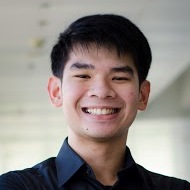
\includegraphics[width=0.2\columnwidth]{Jarabelo}
\documentAuthor{firstname3} \ \documentAuthor{surname3} \ is currently studying B. S. Computer Engineering in De La Salle University, Malate, Manila, Philippines. 

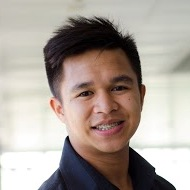
\includegraphics[width=0.2\columnwidth]{Uy}
\documentAuthor{firstname4} \ \documentAuthor{surname4} \ is a forth year engineering student and currently taking up Bachelor of Science in Computer Engineering at De La Salle University - Manila, Philippines. He is knowledgeable in database systems, programming languages such as C, CSS, Java, HTML, MySQL, PHP and Verilog, and has developed several electronic circuits that utilizes the PIC microcontroller. His research interest includes automation, environment friendly technologies and radio frequency identification technologies.

%\vfill
%}

